\section{The model}
\label{sec:md_model}
The state of a Molecular Dynamics system is fully described by seven variables per atom; three positions, three velocities plus the atom type. The phase variables are evolved through the laws of motion. It is here common, as in DSMC (see section \ref{sec:dsmc_model}), to apply periodic boundary conditions. Applied periodic boundary conditions in all directions implies constant volume (unless, of course, we rescale the system size which can be done). The atomic forces are calculated as the gradient of a chosen potential that can differ quite a lot depending on the requirements of the model. A noble gas like Argon can be modelled with a simple potential called the Lennard-Jones potential which will be discussed below. With this potential, one can calculate equilibrium thermodynamic properties that are in good agreement with experimental values \cite{verlet1967computer}. System statistics are sampled as ensable averages through ergodicity over large times. A typical Molecular Dynamics algorithm is illustrated in figure \ref{fig:flow_simple_md}.
\begin{figure}[h]
\framebox{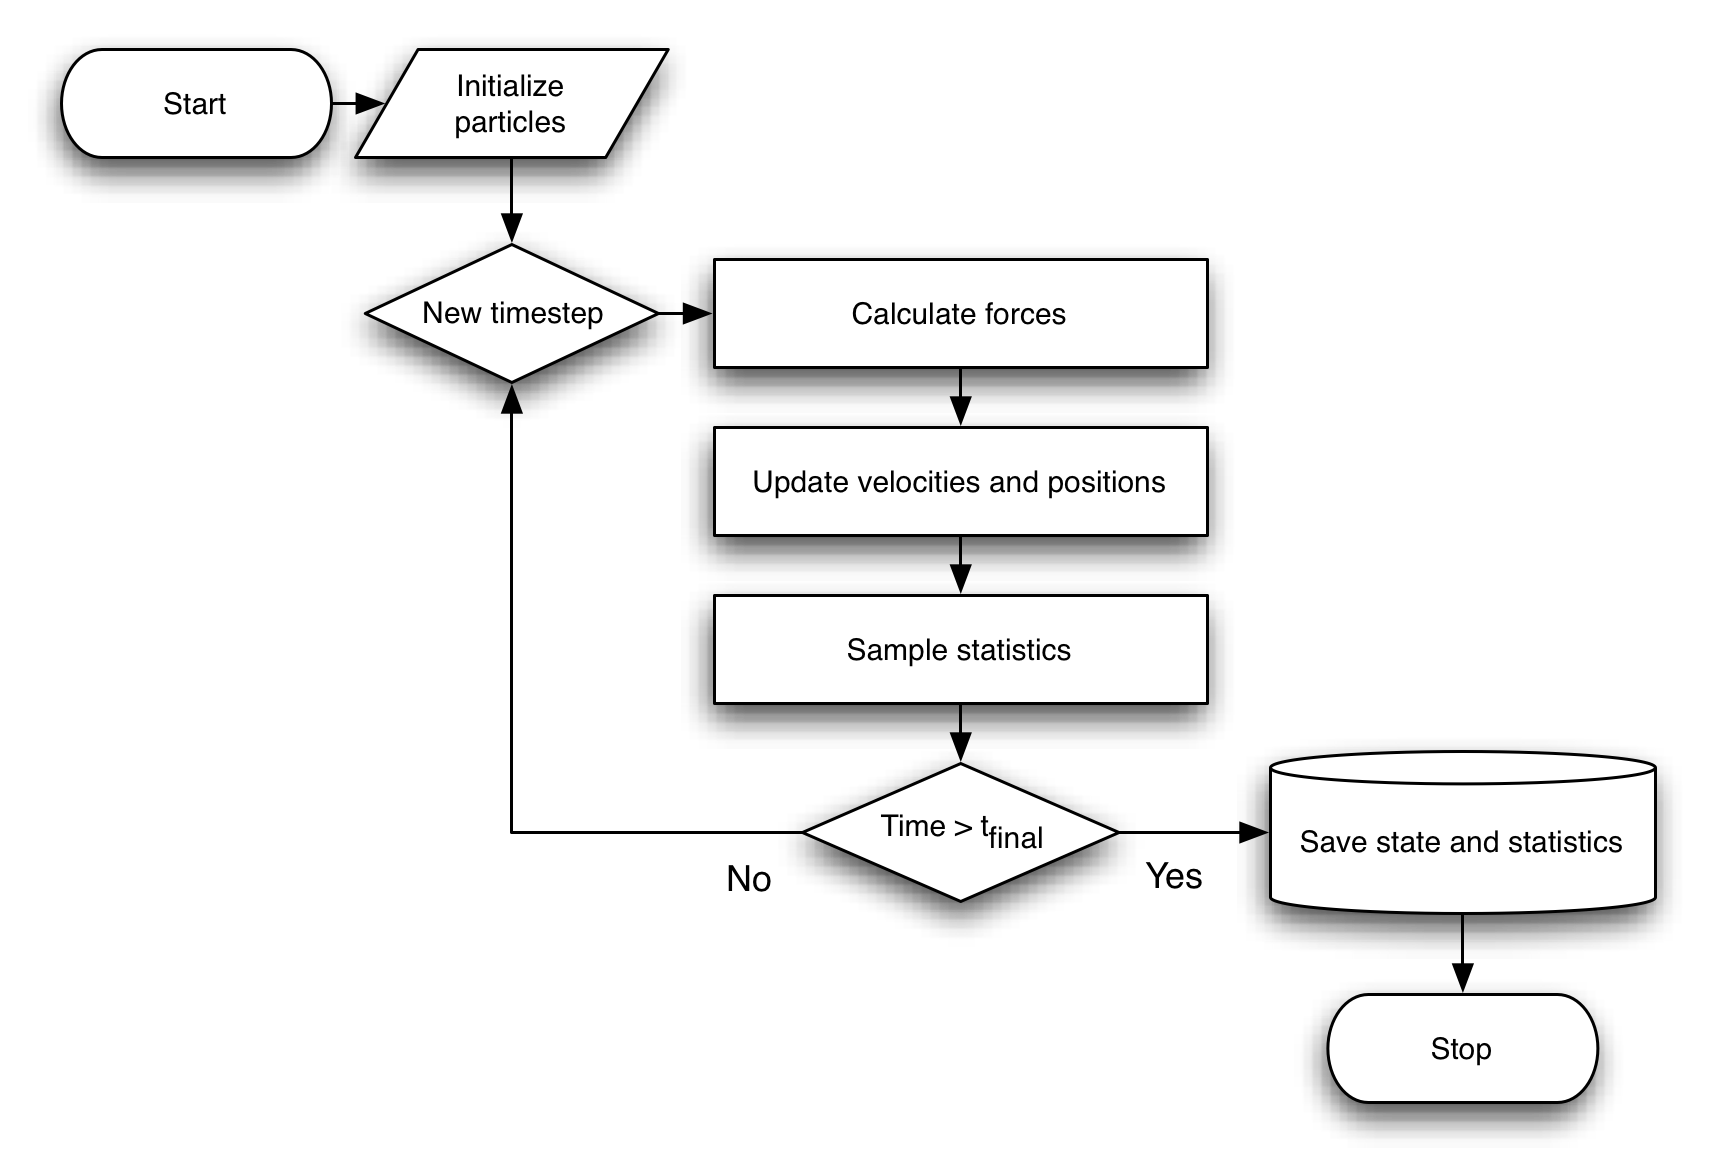
\includegraphics[width=0.8\textwidth, trim=0cm 0cm 0cm 0cm, clip]{MD/figures/SimpleMD.png}}
\centering
\caption{Flow chart illustrating a typical Molecular Dynamics algorithm.}
\label{fig:flow_simple_md}
\end{figure}